\chapter{\IfLanguageName{dutch}{Proof Of Concept}{Proof-Of-Concept}}
\label{ch:proof-of-concept}

In dit gedeelte wordt de data door eigen geschreven code getraind en wordt er geprobeerd om een betere of even goede nauwkeurigheid te behalen op de drie datasets als bij de Azure Text Analytics API en het Google Cloud Platform. Het schrijven en testen van de code, gebeurt aan de hand van de stappen die in sectie \ref{sec:hoewordtdatasetgetraind} besproken werden. Data Preparatie is de eerste stap, daarna Data Cleaning gevolgd door het opzetten van de training en test dataset. In dit onderzoek zullen ook enkele visualisaties van de data gedaan worden om hier een beter begrip van te kunnen vormen. Dit gebeurt in sectie \ref{proofofconceptdataexploratie}, Data Exploratie. Ten slotte wordt het juiste model gekozen en getraind. 

Een belangrijke nota is dat de code gebaseerd is op code gevonden op de website Kaggle.com. Kaggle is een website waar er veel datasets te vinden zijn die de gebruiker, mits het aanmaken van een account, kan downloaden voor eigen gebruik. Verder kan de gebruiker op de website zelf code schrijven voor deze datasets. Het was enorm interessant om de code van de verschillende gebruikers te evalueren en zelf toe te passen om het best mogelijke model te vinden. \autocite{Kaggle2021}

\section{Data Preparatie}
\label{proofofconceptdatapreparatie}
De eerste stap die met beide datasets ondernomen wordt, is de data preparatie stap. Tijdens deze stap wordt onnodige data verwijderd. De Amazon en de IMDB datasets bevatten geen onnodige data. Wat wel opnieuw moet gebeuren, is het omzetten van de dataset naar bruikbare data. Voor de Twitter dataset zullen enkele kolommen verwijderd moeten worden.

\subsection{Amazon dataset}
Het omzetten van de data uit de Amazon dataset verloopt ongeveer gelijkaardig aan de omzetting die gebeurt in hoofdstuk \ref{amazondatasetomzettenazure}.

Allereerst wordt de data opgehaald via Google Drive. Daarna worden de correcte imports gedeclareerd. Deze stap kan ook gevonden worden in figuur \ref{stap1amazon}. Eenmaal de data ingelezen is, worden de reviews gedecodeerd via de functies readlines() en decode(), zoals ook te zien is op figuur \ref{stap2amazon}. Voor het trainen van de AI, worden enkel de eerste 200.000 reviews gebruikt. Dit wordt ook gedaan omdat de Twitter Dataset heel wat kleiner is dan de Amazon dataset. Op deze manier krijgt men hopelijk een consistenter resultaat. 

Nadat de data gedecodeerd werd, worden de labels uit de tekst getrokken en worden alle url's verwijderd uit de tekst zoals ook te zien in figuren \ref{stap3amazon} en \ref{stap4amazon}. 

Uiteindelijk wordt de data omgezet naar een \gls{dataframe} met zowel de reviews als de scores. Een voorbeeld van hoe de data er nu uitziet, kan gevonden worden in figuur \ref{amazondataframe}.

\begin{figure}[!htbp]
    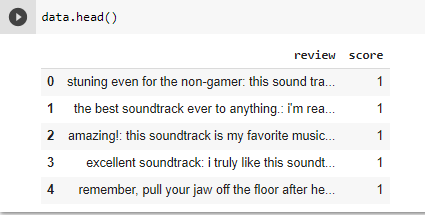
\includegraphics[width=\textwidth]{AI/AmazonDataframe.PNG}
    \caption{\label{amazondataframe}Dataframe voor de Amazon dataset.}
\end{figure}
\FloatBarrier 

\subsection{Twitter dataset}
Het omzetten van de data uit de Twitter dataset verloopt ook gelijkaardig aan de omzetting die gebeurt in hoofdstuk \ref{twitterdatasetomzettenazure}

De data wordt opnieuw opgehaald via Google Drive. De correcte imports worden gedeclareerd en de data wordt ingelezen zoals in figuur \ref{azurestap1twitter}

\subsection{IMDB dataset}
Ook het omzetten van de data uit de IMDB dataset verloopt gelijkaardig aan de omzetting die gebeurt in hoofdstuk \ref{imdbdatasetomzettenazure}.
Na het declareren van de juiste imports, wordt de data opgehaald via Google Drive. De IMDB dataset bevat maar twee kolommen, namelijk de review kolom die de tekst van de review bevat en de sentiment kolom, die 'positive' of 'negative' bevat. 

\section{Data Cleaning}
\label{proofofconceptdatacleaning}
Een tweede stap is het opschonen van de data. In deze stap worden lege velden verwijderd en wordt niet-numerieke data omgezet in numerieke data.

\subsection{Amazon dataset}
Voor de Amazon dataset is er geen cleaning nodig. De data bestaat momenteel uit de review en de score. Er zijn geen overbodige velden of data die moet omgezet worden. Wat natuurlijk wel nog moet gebeuren is de tekst voorbereiden zodat deze op de meest efficiënte manier door het model kan gaan.

Ten eerste is het handig om uit alle reviews de stopwoorden te verwijderen. Deze hebben immers geen impact op de gevoelswaarden van de review. Dit gebeurt via \gls{tokenization}. Meer info hierover kan gevonden worden in sectie \ref{sec:Tokenization}.

\begin{figure}[!htbp]
    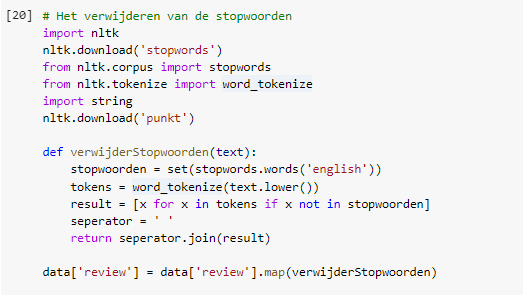
\includegraphics[width=\textwidth]{AI/AmazonTokenization.PNG}
    \caption{\label{amazontokenization}Tokenization voor de Amazon dataset.}
\end{figure}
\FloatBarrier

De data wordt verder verwerkt door er vectors van te maken. Een volledig voorbeeld van de stappen die ondernomen werden is te vinden in bijlage 1.

\subsection{Twitter dataset} 
De Twitter dataset bevat momenteel 15 kolommen, dit is te veel en helemaal niet nodig. De aanmaakdatum, locatie, reden, id,... zijn allemaal velden die niet nodig zijn. Daarom is het de bedoeling om deze tabel om te zetten naar een tabel met enkel de reviews en de scores. 


\begin{figure}[!htbp]
    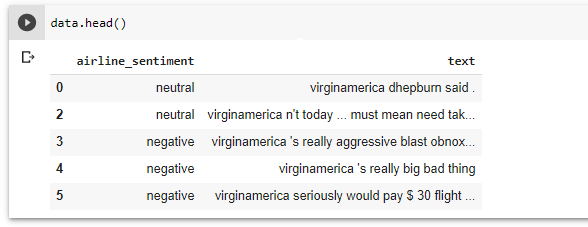
\includegraphics[width=\textwidth]{AI/TwitterData.PNG}
    \caption{\label{twitterdata}Uiteindelijke data voor de Twitter dataset.}
\end{figure}
\FloatBarrier

Voor het verwijderen van de stopwoorden, wordt dezelfde functie als bij de Amazon dataset gebruikt. Deze functie kan gevonden worden in figuur \ref{amazontokenization}. Er is één klein verschil, bij de Twitter dataset moeten de apenstaartjes vooraan de tweets ook verwijderd worden. 

Een tweede omzetting die moet gebeuren, is het omzetten van de woorden 'negatief', 'neutraal' en 'positief' naar 0, 1 en 2. Dit gebeurt aan de hand van onderstaande omzetting:

\begin{figure}[!htbp]
    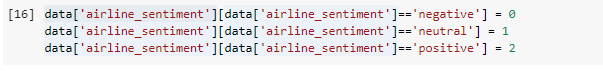
\includegraphics[width=\textwidth]{AI/TwitterOmzetting.PNG}
    \caption{\label{twitteromzetting}Het omzetten van de scores voor de Twitter dataset.}
\end{figure}
\FloatBarrier

\subsection{IMDB dataset}
Voor de IMDB dataset moeten de stopwoorden ook verwijderd worden. Dit is dezelfde functie als in figuur \ref{amazontokenization}. Daarna moeten de woorden 'negative' en 'positive' omgezet worden naar 0 en 1. Deze functie kan men ook vinden in figuur \ref{stap2imdb}. Zoals eerder vermeld, bevat de tekst nog html tags. Deze worden eruit gehaald. Dit gebeurt ook in figuur \ref{stap2imdb}.


\section{Data Exploratie}
\label{proofofconceptdataexploratie}
Dit is een extra toegevoegde stap om eens te gaan kijken wat er juist in de data zit. Dit kan gevisualiseerd worden aan de hand van grafieken, of extra velden. 

\subsection{Amazon dataset}
Om een beter begrip te krijgen van de Amazon dataset, kan men dit op allerlei manieren visualiseren. Momenteel is de Amazon dataset een dataframe. Hierop kan men bijvoorbeeld de functie describe() toepassen. Deze functie toont het aantal rijen data, de gemiddelde score, de \gls{standaardafwijking} (std) en andere gegevens zoals het minimum en het maximum. 

\begin{figure}[!htbp]
    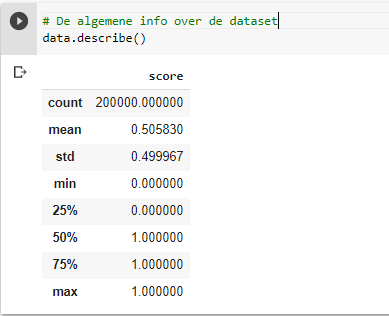
\includegraphics[width=\textwidth]{AI/AmazonDescribe.PNG}
    \caption{\label{amazondescribe}Algemene info over de Amazon dataset.}
\end{figure}
\FloatBarrier 

Hier kan men zien dat er 200.000 rijen data zijn. Het gemiddelde van de data is 0.505, dit betekent dat er een mooie verdeling is tussen positieve en negatieve scores. Het minimum is uiteraard 0 en het maximum is 1. Via de functie data.shape kunnen de dimensies van de data opgevraagd worden. Voor deze dataset is dit (200000,2). De dataset heeft dus 200.000 rijen en twee kolommen. Deze twee kolommen zijn de reviews en de scores. 

Een andere manier om de verdeling tussen de positieve en de negatieve reviews te bekijken, is via een staafdiagram. Deze kan gezien worden in figuur \ref{amazonverdeling} Men kan zien dat er een mooie verdeling is tussen de positieve (oranje balkje) en de negatieve reviews (blauw balkje). Er zijn echter iets meer positieve dan negatieve reviews.

\begin{figure}[!htbp]
    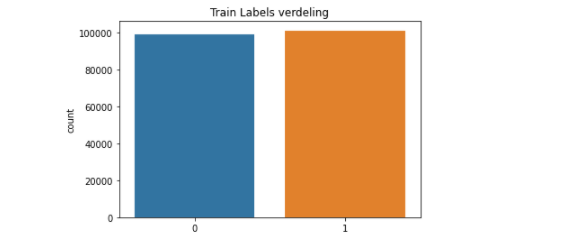
\includegraphics[width=\textwidth]{AI/AmazonVerdeling.PNG}
    \caption{\label{amazonverdeling}Verdeling van de Amazon dataset.}
\end{figure}
\FloatBarrier 

Verder kan ook gekeken worden hoeveel woorden en hoeveel karakters een gemiddelde review bevat en wat de \gls{density} van de reviews is. De density wordt berekend door het aantal woorden door het aantal karakters te delen. Hierdoor geldt het principe dat hoe kleiner de density is, hoe langer de verschillende woorden in de review zijn. 

\begin{figure}[!htbp]
    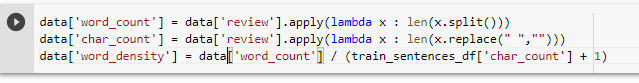
\includegraphics[width=\textwidth]{AI/AmazonExtraVelden.PNG}
    \caption{\label{amazonaantalwoorden}Extra velden voor de Amazon dataset.}
\end{figure}
\FloatBarrier

De resultaten van deze nieuwe kolommen kunnen gevonden worden in figuur \ref{amazondescribe2}.

\begin{figure}[!htbp]
    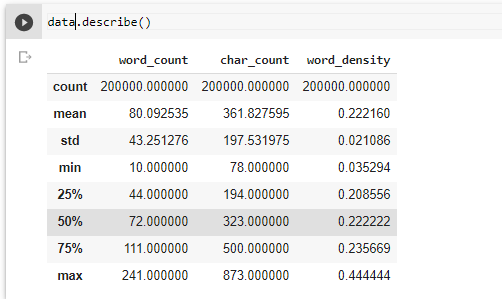
\includegraphics[width=\textwidth]{AI/AmazonDescribe2.PNG}
    \caption{\label{amazondescribe2}Algemene info over de Amazon dataset.}
\end{figure}
\FloatBarrier

Ook hier kan de functie describe op toegepast worden. Het gemiddeld aantal woorden is 80,09, het minimum aantal woorden is 10 en het maximum aantal woorden is 241. Onder de kolom char\_count, kan men zien hoeveel karakters een review gemiddeld bevat. Een review bevat gemiddeld 361.82 karakters, het minimum aantal karakters van een review is 78 en het maximum is 873 karakters. Deze dataset heeft dus een grote variatie aan reviews. Dit kan ook afgeleid worden uit de word\_density, waar het gemiddelde 0.22 is, het minimum 0.035 is en het maximum 0.44 is.

Deze data kan ook in een grafiek gegoten worden.

\begin{figure}[!htbp]
    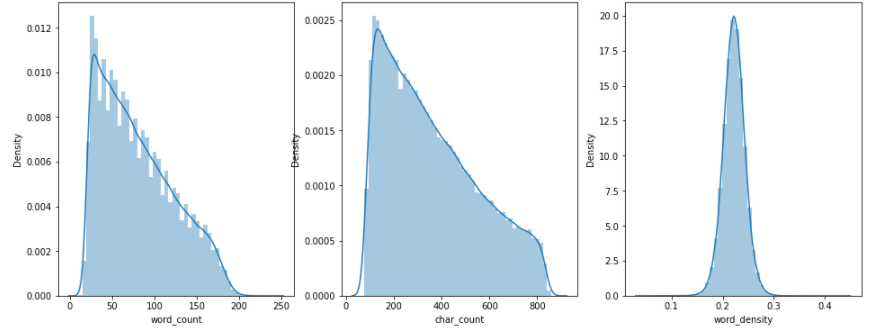
\includegraphics[width=\textwidth]{AI/AmazonExtraGrafiek.PNG}
    \caption{\label{amazongrafiek}Een grafiek over het aantal woorden, karakters en de density van de Amazon dataset.}
\end{figure}
\FloatBarrier


De grafieken zien er alle drie anders uit. Voor het aantal woorden en het aantal karakters springt direct in het oog dat er een grote varieteit is. Dit kan men zien aan de breedte van de grafiek die zich uitstrekt van het minimum tot het maximum. De \gls{density} voor de reviews blijft redelijk dezelfde voor alle reviews. 


\subsection{Twitter dataset}
Voor de Twitter dataset, kan de data ook eens geanalyseerd en gevisualiseerd worden. Na de omzetting kan de score drie betekenissen aannemen. Negatief wordt 0, neutraal wordt 1 en positief wordt 1. Het is dan duidelijk dat het minimum van deze dataset 0 is en het maximum 2 is. Het gemiddelde van de dataset is 0.32. Dit gemiddelde ligt niet zo mooi in het midden als de Amazon dataset. De verdeling van de Twitter dataset is namelijk minder goed. 

Deze verdeling kan ook eens in een grafiek getoond worden.

\begin{figure}[!htbp]
    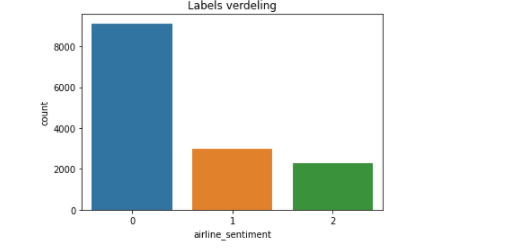
\includegraphics[width=\textwidth]{AI/TwitterVerdeling.PNG}
    \caption{\label{twittergrafiek}Verdeling van de Twitter dataset.}
\end{figure}
\FloatBarrier

Men kan duidelijk zien dat er veel meer negatieve tweets zijn dan neutrale en positieve. Dit kan ervoor zorgen dat de data iets minder betrouwbaar zal zijn. Zoals eerder vermeld zijn tweets ook meestal korter. Dit kan gecontroleerd worden door de functie describe() toe te passen op enkele extra aangemaakte velden.

\begin{figure}[!htbp]
    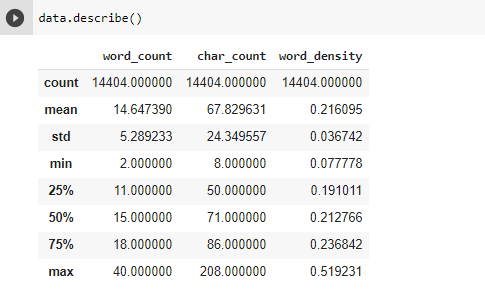
\includegraphics[width=\textwidth]{AI/TwitterExtraData2.PNG}
    \caption{\label{twitterextradata}Extra velden voor de Twitter dataset.}
\end{figure}
\FloatBarrier

Er is een duidelijke tendens zichtbaar. Ten eerste is de omvang van de dataset veel kleiner dan bij de Amazon dataset. De Twitter dataset telt maar 14.404 tweets, terwijl de Amazon dataset 200.000 reviews bevat. Het gemiddeld aantal woorden per tweet is 14. Dit is enorm laag, zeker vergeleken met de Amazon dataset. Het maximum aantal woorden is 40 en het minimum aantal woorden is 2. 
Kan dit een probleem vormen? Is de dataset daarom minder betrouwbaar? Reviews en tweets komen in alle vormen en maten. Een goede AI moet zowel korte als lange reviews/tweets kunnen analyseren. Daarom is het goed om drie compleet verschillende datasets met elkaar te vergelijken. 

Het aantal woorden, karakters en de density kunnen opnieuw in een grafiek geplaatst worden.

\begin{figure}[!htbp]
    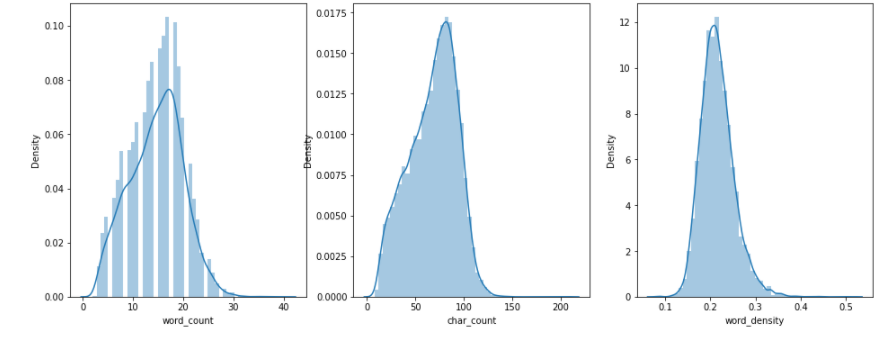
\includegraphics[width=\textwidth]{AI/TwitterExtraGrafiek.PNG}
    \caption{\label{twitterextragrafiek}Een grafiek over het aantal woorden, karakters en de density van de Twitter dataset.}
\end{figure}
\FloatBarrier

\subsection{IMDB dataset}
Dankzij de functie data.describe(), wordt vastgesteld dat de dataset 50.000 reviews bevat. De omvang van de dataset is dan ook (50.000,2).

Om de verdeling van de dataset te beoordelen, wordt dit in een grafiek gegoten. Er blijken evenveel negatieve (blauwe balkje) als positieve (oranje balkje) reviews te zijn. Dit is heel goed, dit betekent dat de IMDB dataset een heel evenwichtige dataset is. 

\begin{figure}[!htbp]
    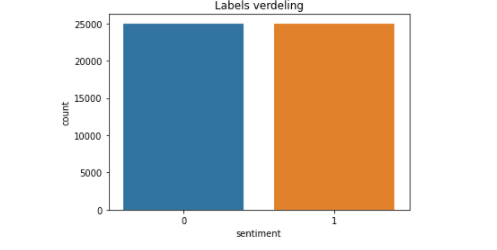
\includegraphics[width=\textwidth]{AI/IMDBVerdeling.PNG}
    \caption{\label{imdbgrafiek}Verdeling van de IMDB dataset.}
\end{figure}
\FloatBarrier

Daarna kunnen opnieuw de extra velden word\_count, char\_count en word\_density toegevoegd worden. 

\begin{figure}[!htbp]
    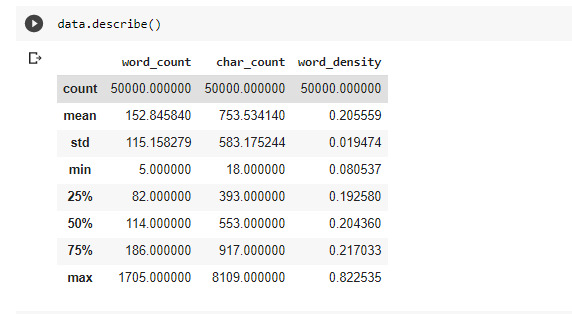
\includegraphics[width=\textwidth]{AI/IMDBExtraData.PNG}
    \caption{\label{imdbextradata}Extra data voor de IMDB dataset.}
\end{figure}
\FloatBarrier

Het gemiddeld aantal woorden is 152.84, met als maximum aantal woorden 1705 en minimum aantal woorden 5. Deze getallen liggen enorm uiteen. Ook het aantal karakters kan afgeleid worden uit bovenstaande tabel. Het gemiddeld aantal karakters is 752, met een maximum van 8109 karakters en een minimum van 18 karakters. De density wordt berekend door het aantal woorden te delen door het aantal karakters. Hoe lager de density, hoe langer de woorden in de review. Het density-gemiddelde is 0.20, het minimum is 0.08 en het maximum is 0.82. Opnieuw liggen deze getallen ver uiteen. Wanneer deze data in een grafiek gegoten wordt, valt dit helemaal niet op.

\begin{figure}[!htbp]
    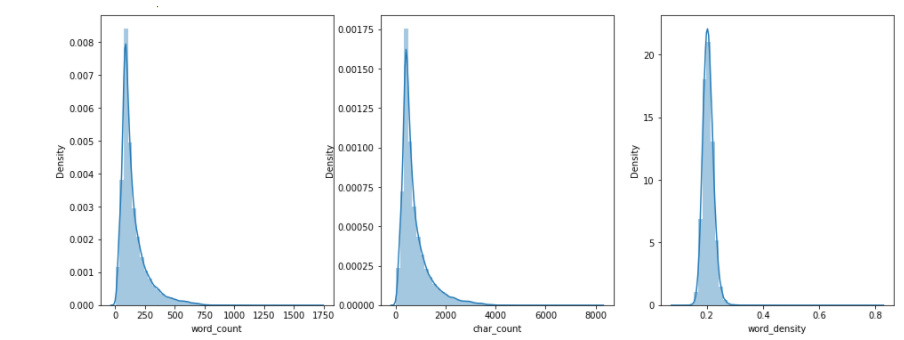
\includegraphics[width=\textwidth]{AI/IMDBExtraGrafiek.PNG}
    \caption{\label{imdbextragrafiek}Een grafiek voor het aantal woorden, karakters en de density van de IMDB dataset.}
\end{figure}
\FloatBarrier

De lengte van de reviews, het aantal karakters en de density ligt voor alle reviews ongeveer bij elkaar. Dit kan geconcludeerd worden uit het feit dat de grafieken niet wijd zijn. Alle data ligt geconcentreerd. De dataset bevat echter wel enkele uitschieters. Daarom dat de maxima en minima zo ver uiteen liggen. 


\section{Opzetten van training dataset en test dataset}
De dataset wordt hier opgesplitst. 70\% van de data wordt training dataset en 30\% van de data wordt test dataset. Dit gebeurt voor alle datasets op dezelfde manier.

\begin{figure}[!htbp]
    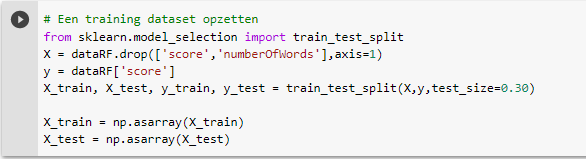
\includegraphics[width=\textwidth]{AI/AmazonValidatie.PNG}
    \caption{\label{amazonopsplitsing}Opsplitsen training en test dataset.}
\end{figure}
\FloatBarrier

\section{Model kiezen}
\label{proofofconceptdatamodel}
Het is enorm moeilijk om het juiste model te kiezen. Een extra laag of epoch kan een groot verschil uitmaken in de nauwkeurigheid van het model. 

\subsection{Model 1}

Een eerste model dat getest wordt, is een \gls{CNN} model: een Convolutional Neural Network. Na enkele testen blijkt dat voor de Amazon dataset 30 epochs meer dan genoeg zijn, terwijl de Twitter dataset betere resultaten toont bij 50 epochs.
\begin{figure}[!htbp]
    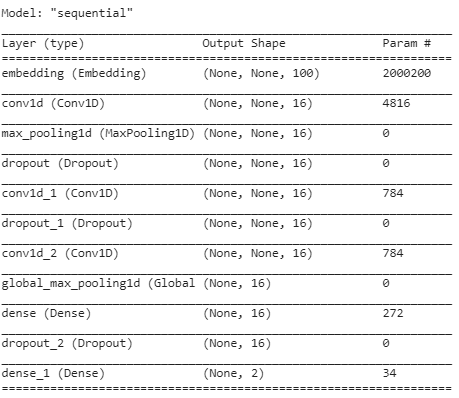
\includegraphics[width=\textwidth]{AI/Model1.PNG}
    \caption{\label{model1}Model 1}
\end{figure}
\FloatBarrier

\begin{figure}[!htbp]
    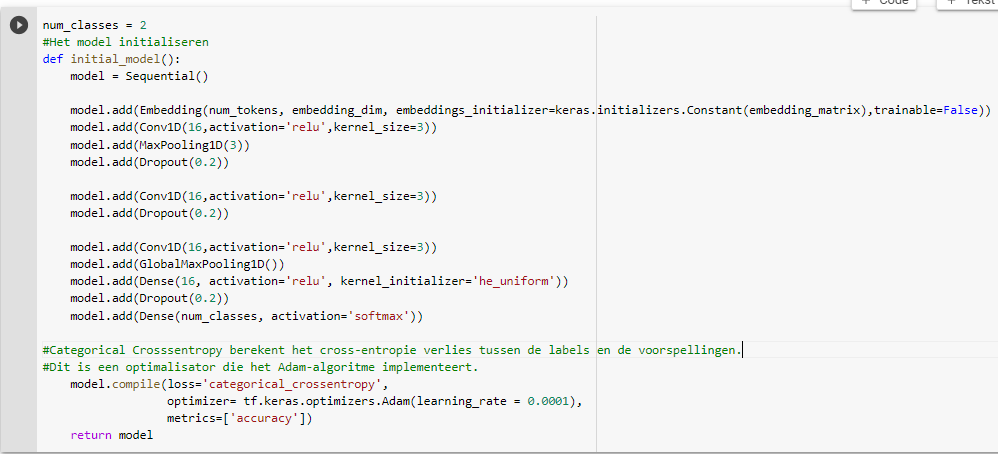
\includegraphics[width=\textwidth]{AI/Model1-2.PNG}
    \caption{\label{model1.2}Model 1}
\end{figure}
\FloatBarrier

Zoals gezien kan worden op figuur \ref{model1}, is het model een sequentieel model. Dit model wordt gebruikt voor een 'stapel' lagen. Elke laag heeft 1 input en 1 output. Daarom wordt hier sequentieel doorgegaan. Het is ook duidelijk dat er een aantal verschillende lagen gebruikt worden. Zowel convolutional layers, dense layers als pooling layers worden hier gebruikt. Meer informatie over deze verschillende lagen kan gevonden worden in sectie \ref{sec:neuralnetworks}. 

Laag 1: Embedding laag: Zet alle positieve getallen, in dit geval de scores om naar vectors. \\
Laag 2: Convolutionele laag met 16 filters en met als activatiefunctie de ReLU, met kernel\_size gelijk aan 3. \\
De kernel size is eigenlijk de grootte van de filter die over de data geschoven wordt. \\
Laag 3: MaxPooling1D: Een pooling layer met lengte 3. In deze laag wordt steeds het maximum berekend van elke feature. Een pooling layer bevindt zich steeds bij een convolutionele laag. \\
Laag 4: Dropout laag met een frequentie van 0.2. Wordt gebruikt om overfitting te vermijden. \\
Laag 5: Convolutionele laag met 16 filters, activatiefunctie ReLU en kernel\_size gelijk aan 3. \\
Laag 6: Dropout laag met een frequentie van 0.2. \\
Laag 7: Convolutionele laag met 16 filters, de ReLU activatiefunctie en kernel\_size 3. \\
Laag 8: GlobalMaxPooling1D laag: een pooling layer die het maximum berekent voor het volledige model. \\
Laag 9: Dense laag: Volledig verbonden laag met 16 filters, een ReLU activatiefunctie en een he\_uniform initializer. \\
Een kernel initializer bepaalt welke verdeling of functie gebruikt moet worden om de gewichten te initialiseren. \\
Laag 10: Dropout laag met een frequentie van 0.2. \\
Laag 11: Dense laag met als output het aantal klassen en activatiefunctie \gls{softmax}. \\
De softmax activatiefunctie wordt gebruikt om de data terug te normaliseren, daarom wordt deze op het einde gebruikt.   

Het duurt even om het model te trainen, maar na een tijdje komen hier resultaten uit. 

Voor de Amazon dataset heeft dit model een nauwkeurigheid van 82\%. Deze worden in een grafiek gestoken zodat men het verloop van de training gedurende de verschillende epochs kan zien. 

\begin{figure}[!htbp]
    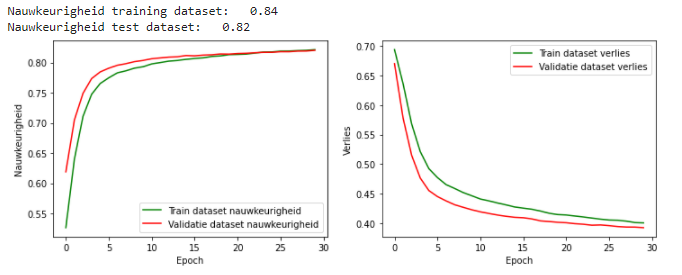
\includegraphics[width=\textwidth]{AI/AmazonResult.PNG}
    \caption{\label{amazonresult}Resultaten Model 1 Amazon dataset.}
\end{figure}
\FloatBarrier

Voor de Twitter dataset heeft dit model een nauwkeurigheid van 75\%
Een belangrijke nota hierbij is dat de Twitter dataset 50 epochs nodig had, terwijl de Amazon dataset 30 epochs nodig had.

Wat is de reden hiervoor?
De Twitter dataset bevat minder data en dus moet de AI aan de hand van minder voorbeelden trainen. Wanneer het aantal epochs verhoogd wordt, doorloopt de AI deze cyclus 50 keer. 
Ook deze resultaten zijn te vinden in een grafiek zoals te zien op figuur \ref{twitterresult}. 

\begin{figure}[!htbp]
    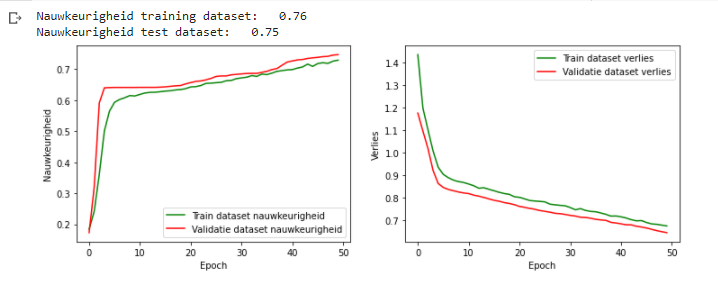
\includegraphics[width=\textwidth]{AI/TwitterResult.PNG}
    \caption{\label{twitterresult}Resultaten Model 1 Twitter dataset.}
\end{figure}
\FloatBarrier

Voor de IMDB dataset heeft dit model een nauwkeurigheid van 72\%.
Ook de IMDB dataset had 50 epochs nodig om een goed resultaat weer te geven. De IMDB dataset bevat ook minder reviews dan de Amazon dataset, dus zijn er meer epochs nodig. Deze resultaten zijn te vinden in de grafiek van figuur \ref{imdbresult}

\begin{figure}[!htbp]
    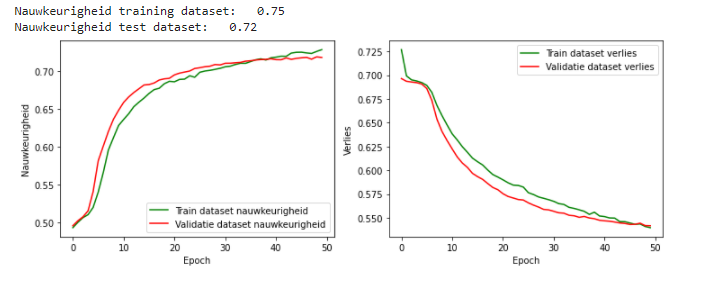
\includegraphics[width=\textwidth]{AI/IMDBResult.PNG}
    \caption{\label{imdbresult}Resultaten Model 1 IMDB dataset.}
\end{figure}
\FloatBarrier

\subsection{Model 2}
In het tweede model werd een andere volgorde van lagen gehanteerd en was het aantal lagen ook minder. Model 2 bleef wel nog steeds een \gls{CNN}. 
Laag 1 is opnieuw een Embedding laag, gevolgd door een Convolutional layer, een GlobalMaxPooling layer en een Dense layer.
Als optimizer wordt opnieuw adam gebruikt.

\begin{figure}[!htbp]
    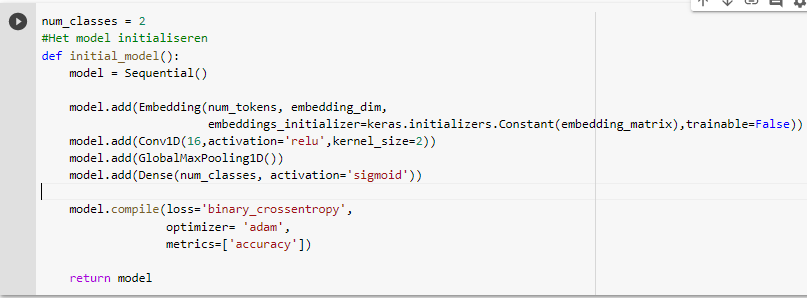
\includegraphics[width=\textwidth]{Models/Model2OverfittingModel.PNG}
    \caption{\label{overfitting} Model 2.}
\end{figure}
\FloatBarrier

Bij dit model bleek er echter overfitting te zijn. Dit kan men zien doordat er een groot verschil is in de grafiek tussen de training en test dataset nauwkeurigheid.

\begin{figure}[!htbp]
    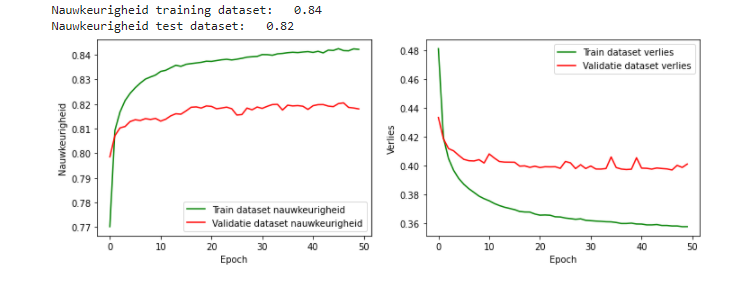
\includegraphics[width=\textwidth]{Models/Model2AmazonResult.PNG}
    \caption{\label{overfittingresult} Resultaten Model 2 Amazon dataset: overfitting.}
\end{figure}
\FloatBarrier

Daarom was het verstandig om enkele \gls{dropoutlaag} toe te voegen. Dropout lagen vermijden overfitting. Model 2 zag er daardoor als volgt uit:

\begin{figure}[!htbp]
    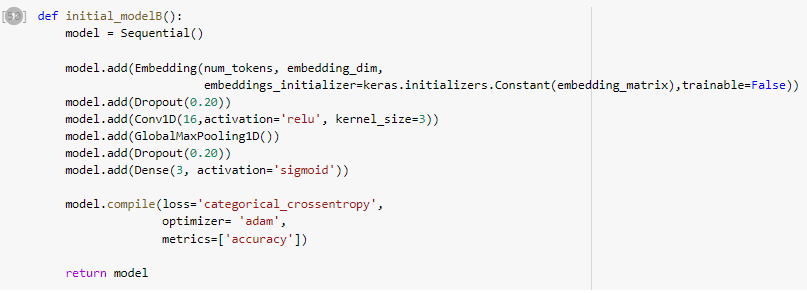
\includegraphics[width=\textwidth]{Models/Model2.PNG}
    \caption{\label{model2.1} Model 2.1.}
\end{figure}
\FloatBarrier

\begin{figure}[!htbp]
    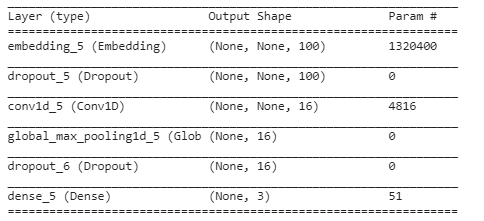
\includegraphics[width=\textwidth]{Models/Model2Summary.PNG}
    \caption{\label{model2.1summary} Model 2.1.}
\end{figure}
\FloatBarrier


Dit model werd dan op de drie datasets toegepast. Voor de eerste dataset, de Amazon dataset, behaalde dit model een nauwkeurigheid van 82\% Op de test dataset.

\begin{figure}[!htbp]
    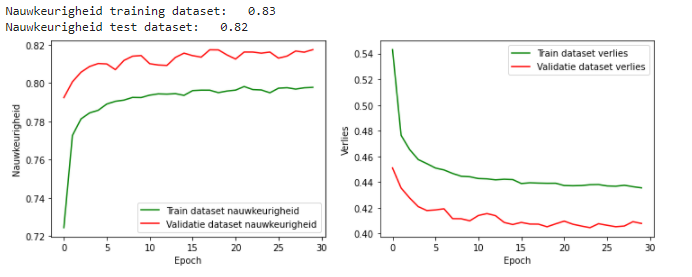
\includegraphics[width=\textwidth]{Models/Model2-1AmazonResult.PNG}
    \caption{\label{amazonresult2}Resultaten Model 2 Amazon dataset.}
\end{figure}
\FloatBarrier

Model 2 behaalde voor de Twitter dataset een nauwkeurigheid van 78\%.

\begin{figure}[!htbp]
    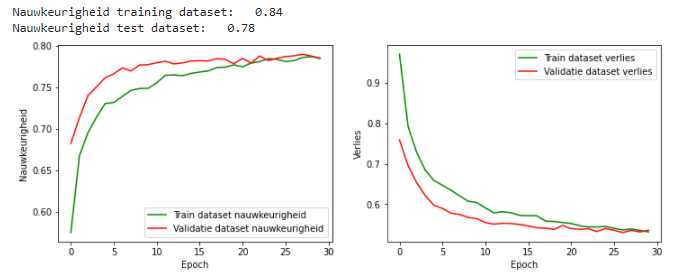
\includegraphics[width=\textwidth]{Models/Model2-1TwitterResult.PNG}
    \caption{\label{twitterresult2}Resultaten Model 2 Twitter dataset.}
\end{figure}
\FloatBarrier

Voor de IMDB dataset werd een nauwkeurigheid van 73\% behaald.

\begin{figure}[!htbp]
    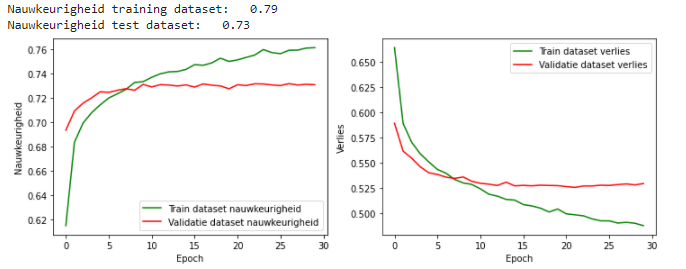
\includegraphics[width=\textwidth]{Models/Model2-1IMDBResult.PNG}
    \caption{\label{imdbresult2}Resultaten Model 2 IMDB dataset.}
\end{figure}
\FloatBarrier

\subsection{Model 3}

Model 3 is opnieuw een Sequentieel model met als eerste laag een Embeddingslaag zodat de embeddings matrix gemakkelijk kan toegevoegd worden.

\begin{figure}[!htbp]
    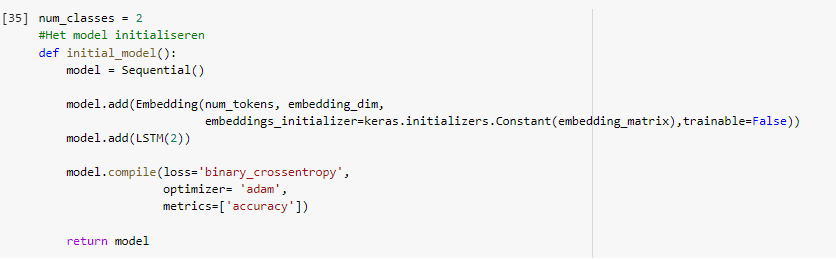
\includegraphics[width=\textwidth]{Models/Model3Amazon.PNG}
    \caption{\label{model3}Model 3.}
\end{figure}
\FloatBarrier

Laag 2 bestaat uit een LSTM laag met 2 parameters. LSTM staat voor Long short-term memory en is een voorbeeld van een \gls{RNN}: Recurrent Neural Network. LSTM bevat feedbackverbindingen waarbij bij elke stap beslist zal worden welke data er bewaard wordt en welke vergeten wordt. 
\begin{figure}[!htbp]
    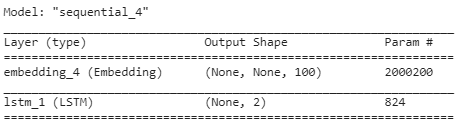
\includegraphics[width=\textwidth]{Models/Model3Amazon2.PNG}
    \caption{\label{model3.2}Model 3.}
\end{figure}
\FloatBarrier

Dit model werd op drie datasets toegepast. Voor de Amazon dataset had dit model een nauwkeurigheid van 82\%

\begin{figure}[!htbp]
    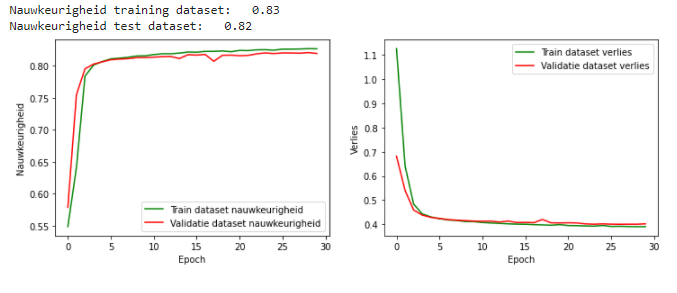
\includegraphics[width=\textwidth]{Models/Model3AmazonResult.PNG}
    \caption{\label{model3amazon}Resultaten Model 3 Amazon dataset.}
\end{figure}
\FloatBarrier

Model 3 leverde voor de Twitter dataset een nauwkeurigheid van 76\% op.

\begin{figure}[!htbp]
    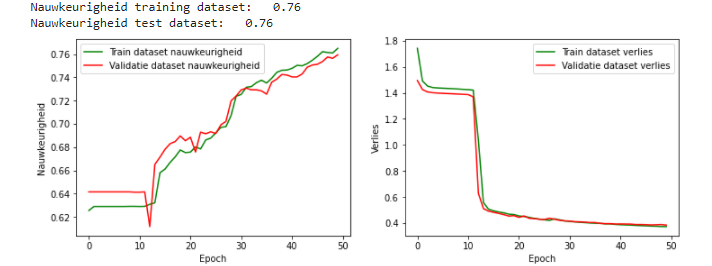
\includegraphics[width=\textwidth]{Models/Model3TwitterResult.PNG}
    \caption{\label{model3twitter}Resultaten Model 3 Twitter dataset.}
\end{figure}
\FloatBarrier

Ten slotte, voor de IMDB dataset werd er een nauwkeurigheid van 72\% geteld.

\begin{figure}[!htbp]
    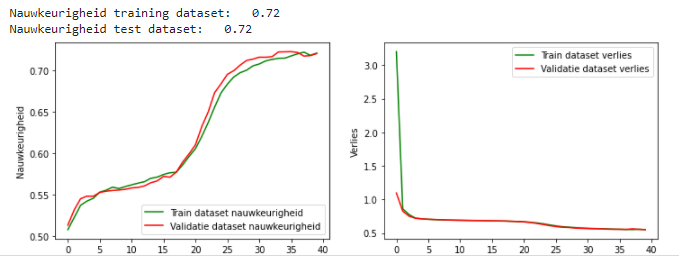
\includegraphics[width=\textwidth]{Models/Model3IMDBResult.PNG}
    \caption{\label{model3imdb}Resultaten Model 3 IMDB dataset.}
\end{figure}
\FloatBarrier

\subsection{Model 4}
Een laatste model dat getest werd, is model 4. Model 4 is opnieuw een Sequentieel model met als eerste laag een embedding laag. Naast het feit dat er opnieuw een LSTM (Long short-term memory) laag gebruikt wordt, bevindt deze zich nu in een Bidirectionele laag. Deze laag verbindt twee verborgen lagen die uit een tegengestelde richting komen met eenzelfde output. Het voordeel hiervan is dat deze outputlaag tegelijk de informatie uit het verleden en uit de toekomst bevat. Dit model is opnieuw een RNN (Recurrent Neural Network). Omdat dit in een bidirectionele laag zit, wordt dit ook een BRNN (Bidirectional Recurrent Neural Network) genoemd.

Na deze laag komen er enkele bekende lagen. Een Dense laag met als activatiefunctie ReLU staat op de derde laag. De vierde laag is een Dropoutlaag met 0.50 dropout frequentie. Dit wordt opnieuw gebruikt om overfitting te vermijden. Laag 5 is opnieuw een Dense laag, maar met als activatiefunctie de softmax.

\begin{figure}[!htbp]
    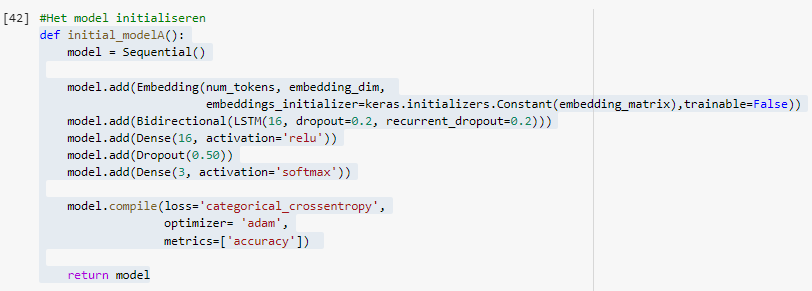
\includegraphics[width=\textwidth]{Models/Model4.PNG}
    \caption{\label{model4}Model 4.}
\end{figure}
\FloatBarrier

De drie datasets werden opnieuw door dit model getraind. 30 epochs bleek hier de beste resultaten op te leveren. Voor de Amazond dataset leverde model 4 een nauwkeurigheid van 85\% op.

\begin{figure}[!htbp]
    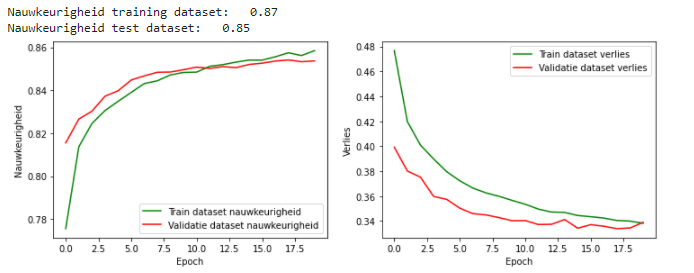
\includegraphics[width=\textwidth]{Models/Model4AmazonResult.PNG}
    \caption{\label{model4amazon}Resultaten Model 4 Amazon dataset.}
\end{figure}
\FloatBarrier

Voor de Twitter dataset behaalde model 4 een nauwkeurigheid van 80\%.

\begin{figure}[!htbp]
    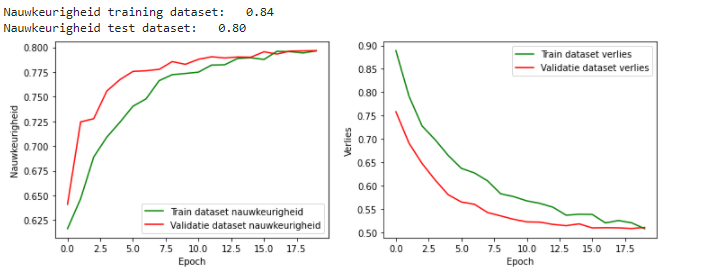
\includegraphics[width=\textwidth]{Models/Model4TwitterResult.PNG}
    \caption{\label{model4twitter}Resultaten Model 4 Twitter dataset.}
\end{figure}
\FloatBarrier

Ten slotte behaalde model 4 voor de IMDB dataset een nauwkeurigheid van 75\%.

\begin{figure}[!htbp]
    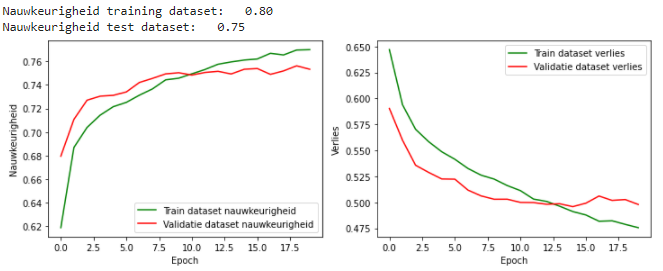
\includegraphics[width=\textwidth]{Models/Model4IMDBResult.PNG}
    \caption{\label{model4imdb}Resultaten Model 4 IMDB dataset.}
\end{figure}
\FloatBarrier

\section{Samenvatting}
Om de resultaten van alle modellen te kunnen vergelijken, staan deze opgesomd in onderstaande tabel (zie tabel \ref{tab:samenvattingproofofconcept}). Men kan zien dat elk model redelijk goede gemiddelde scores behaalde. Uit de tabel 'Totaal' leidt men af dat model 4 de beste resultaten behaalde, zowel op de Amazon dataset, de Twitter dataset als op de IMDB dataset.

Ondanks dat de resultaten van model 2 redelijk goed waren, treedt er hier en daar wat overfitting op. Model 2 is daarom niet het juiste model om reviews te kunnen analyseren. Model 4 blijft het beste model om NLP toe te passen.


\begin{table}[htb]
    \centering
    \begin{tabular}{@{}llllll@{}}
        \toprule
        & Type Neural Network & Amazon & Twitter & IMDB & Totaal \\ \midrule
        Model 1 & \gls{CNN}                 & 82\%                  & 75\%                   & 72\%                & 76.3\% \\
        Model 2 & CNN                 & 82\%                  & 78\%                   & 73\%                & 77.6\% \\
        Model 3 & \gls{RNN}                 & 82\%                  & 76\%                   & 72\%                & 76.6\% \\
        Model 4 & RNN                 & 85\%                  & 80\%                   & 75\%                & 80\%   \\ \bottomrule
    \end{tabular}
    \caption{Samenvatting resultaten proof of concept}
    \label{tab:samenvattingproofofconcept}
\end{table}
\FloatBarrier
